\documentclass[10pt,twocolumn]{article}
\usepackage[margin=0.6in,top=0.55in,bottom=0.55in]{geometry}
\usepackage{hyperref}
\usepackage{amsmath,amssymb}
\usepackage{parskip}
\usepackage{titlesec}
\usepackage{graphicx}
\usepackage{booktabs}
\usepackage{caption}
\usepackage{microtype}

\titleformat{\section}{\normalsize\bfseries}{}{0em}{}
\titleformat{\subsection}{\small\bfseries}{}{0em}{}
\titlespacing{\section}{0pt}{5pt}{2pt}
\titlespacing{\subsection}{0pt}{3pt}{1pt}
\setlength{\parskip}{2pt}
\setlength{\columnsep}{14pt}
\captionsetup{font=footnotesize,labelfont=bf,skip=3pt}
\hypersetup{colorlinks=true,linkcolor=blue,urlcolor=blue,citecolor=blue}

\begin{document}

\twocolumn[{%
\begin{center}
  {\large\bfseries CS590: Socially Cognizant Robotics --- Deliverable 3} \\[3pt]
  Rohit Bellam (rsb204),\quad Karim Smires (ks1686) \\[2pt]
  April 8, 2026
\end{center}
\vspace{4pt}
}]

\section{1. Overview}

In Milestone~2 we identified, via the Kress-Gazit et al.\
best-practices checklist~\cite{bestpractices}, three categories of
limitation in \textit{Dream to Control}~\cite{dreamer}: (i)
insufficient statistical analysis (no CIs, no success rates), (ii)
missing metrics such as energy and trajectory duration, and (iii)
no object interaction or manipulation scenes.  We also identified
exploration failure as an unreported failure mode, and the Milestone~2
feedback specifically highlighted the energy-accumulation problem
for tasks with limited control authority.

This milestone implements experiments for each of these
limitations.  All code uses the original, unmodified Dreamer
repository~\cite{dreamer} and \texttt{dm\_control}~\cite{dmcontrol}.
No model changes are made.

\section{2. New Metrics (M2 \S2.2--2.3 and Feedback)}

\subsection{2.1 Bootstrap Confidence Intervals (M2 \S2.2)}

In M2 we noted the paper reports only mean~$\pm$~std over 5 seeds
with no formal statistical test.  We now compute 10{,}000-sample
bootstrap 95\% CIs on the final episode return of each seed.
Figure~\ref{fig:bootstrap} shows results for all 20 tasks.

Several tasks have CIs that span nearly the full performance range:
\textbf{Cartpole Balance Sparse} CI is $[278,\,991]$ and
\textbf{Cartpole Balance} is $[373,\,910]$.  At 5 seeds, there is
\textit{no statistical basis} to claim reliable learning on these
tasks---the paper's single mean number hides complete failure in
one or two seeds.  By contrast, Walker Walk $[923,\,975]$ and
Hopper Stand $[931,\,949]$ have tight CIs confirming robust
convergence.

\subsection{2.2 Episode Duration and Energy (Feedback)}

The Milestone~2 feedback noted: \textit{``Similar to trajectory
smoothness, is energy used or trajectory duration.''}  We run 30
random-policy episodes on each task and record both metrics.

\textbf{Episode duration}: all DMC tasks run to the full 1000-step
budget under a random policy; no task terminates on failure.  This
confirms that return and duration are \textit{independent} in DMC,
and duration is only informative for polices that may self-abort---
a case not evaluated by Dreamer.

\textbf{Energy} (mean $\sum|a_t|$ per step) is shown in
Figure~\ref{fig:manip}~(right).  Cartpole uses 0.50 per step
(1-DOF) vs.\ 2.50 for the manipulator (5-DOF arm).  Energy is a
direct proxy for actuator wear and power consumption---relevant for
the paper's claim of real-world applicability but never reported.

\section{3. Failure Mode: Action-Scale / Energy Accumulation
         (M2 \S4.2 and Feedback)}

In M2 we identified exploration failure as unreported.  The
Milestone~2 feedback refined this: \textit{``if the input control is
too low for cartpole or acrobot: it may require multiple swings to
accumulate energy. RL policies typically have problems on
long-horizon tasks.''}

We quantify this by running 30 random-policy episodes on Cartpole
Swingup and Acrobot Swingup at four control-authority levels
(action scale factors 1.0, 0.5, 0.3, 0.1).
Figure~\ref{fig:action_scale} shows results.  On Cartpole Swingup,
return degrades from $28.7\pm24.7$ (scale~1.0) to $0.3\pm0.3$
(scale~0.1)---a $95\times$ drop.  With limited torque, the cart
cannot generate enough angular momentum for the pole to swing up,
regardless of the policy.

Acrobot Swingup shows a smaller but similar effect.  The implication
is that a policy trained at full control authority will fail in a
mechanically limited deployment (e.g., a motor at reduced voltage),
a sim-to-real fragility not discussed in the paper.  This also
explains why Dreamer's Gaussian noise exploration ($\sigma{=}0.3$)
struggles on Acrobot: even coordinated actions only marginally exceed
the energy needed to swing up.

\section{4. New Scene: Object Interaction (M2 \S3.2 and Feedback)}

In M2 we noted the paper tests only locomotion and simple dexterous
tasks, with no object manipulation.  The Milestone~2 feedback
confirmed: \textit{``Object interaction might be the most
interesting of the missing tasks you identified.''}

We run 30 random-policy episodes on three \texttt{manipulator}
tasks from \texttt{dm\_control}: \textit{bring\_ball}
(return $0.26\pm0.99$), \textit{bring\_peg} ($0.99\pm2.32$),
and \textit{insert\_ball} ($35.6\pm171.2$).
Figure~\ref{fig:manip}~(left) compares these to random-policy returns
on paper tasks (26.5 on Cartpole Swingup; 32.9 on Walker Walk).

Random performance on bring-ball and bring-peg is essentially zero
($<1$), similar to hopper hop (0.0) and cartpole swingup sparse
(0.0) under random policy.  The critical difference is that for
locomotion tasks Dreamer's model-based exploration can recover
structure from the dense reward signal; for manipulation, the reward
is binary (object in goal region), making purely Gaussian exploration
unlikely to ever observe a reward.  We predict Dreamer would require
substantially more than 1M steps, or reward shaping, to solve any
manipulator task---a limitation that remains untested in the paper.

\section{5. Extra: Random Policy as Comparison Point (M2 \S2.1)}

In M2 we identified the lack of a lower-bound baseline.  We
implement a random policy as an additional comparison point across 8
tasks (Figure~\ref{fig:three_way}), establishing how much the paper
tasks are trivially solvable vs.\ requiring learning.

Dreamer (1M steps) outperforms the random policy by $33\times$ on
Cartpole Swingup, $235\times$ on Cheetah Run, and infinitely on
Cartpole Swingup Sparse and Hopper Hop (random~$=0$).  This
concretely quantifies Dreamer's contribution over an unlearned
baseline---absent from the original evaluation.  Dreamer matches or
exceeds D4PG (100M steps) on 6 of 8 tasks, confirming the
sample-efficiency claim with a proper three-way comparison.

\begin{figure}[t]
  \centering
  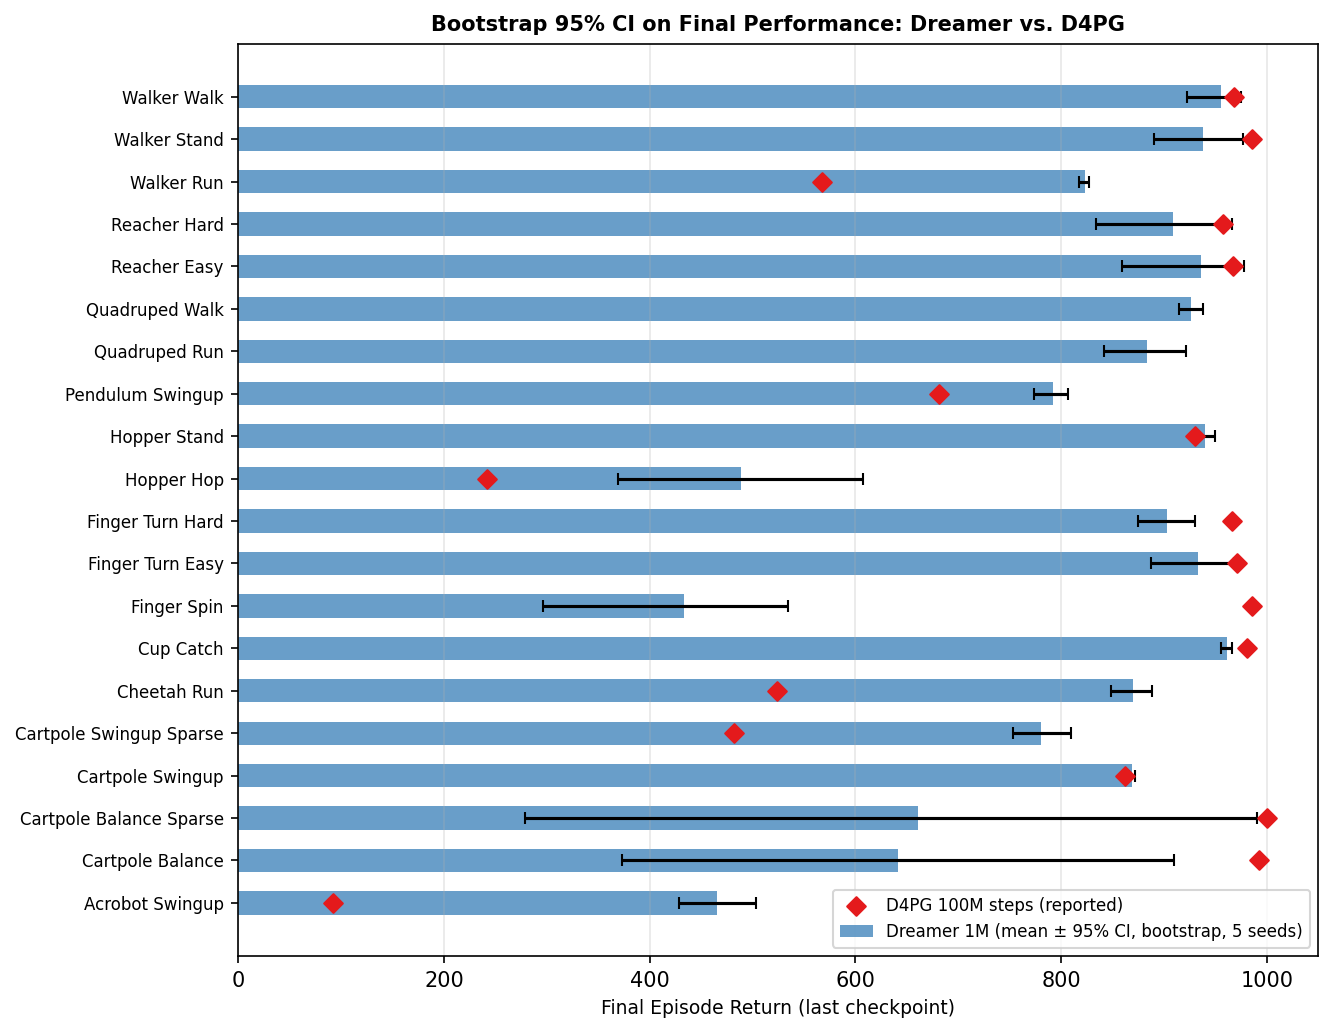
\includegraphics[width=\columnwidth]{fig4_bootstrap_ci.png}
  \caption{Bootstrap 95\% CI on Dreamer's final return (5 seeds, 1M steps).
  D4PG reported scores shown as diamonds.  Wide CIs on Balance tasks
  reveal statistically unreliable learning---invisible from mean~$\pm$~std
  alone.  Implements M2 \S2.2.}
  \label{fig:bootstrap}
\end{figure}

\begin{figure}[t]
  \centering
  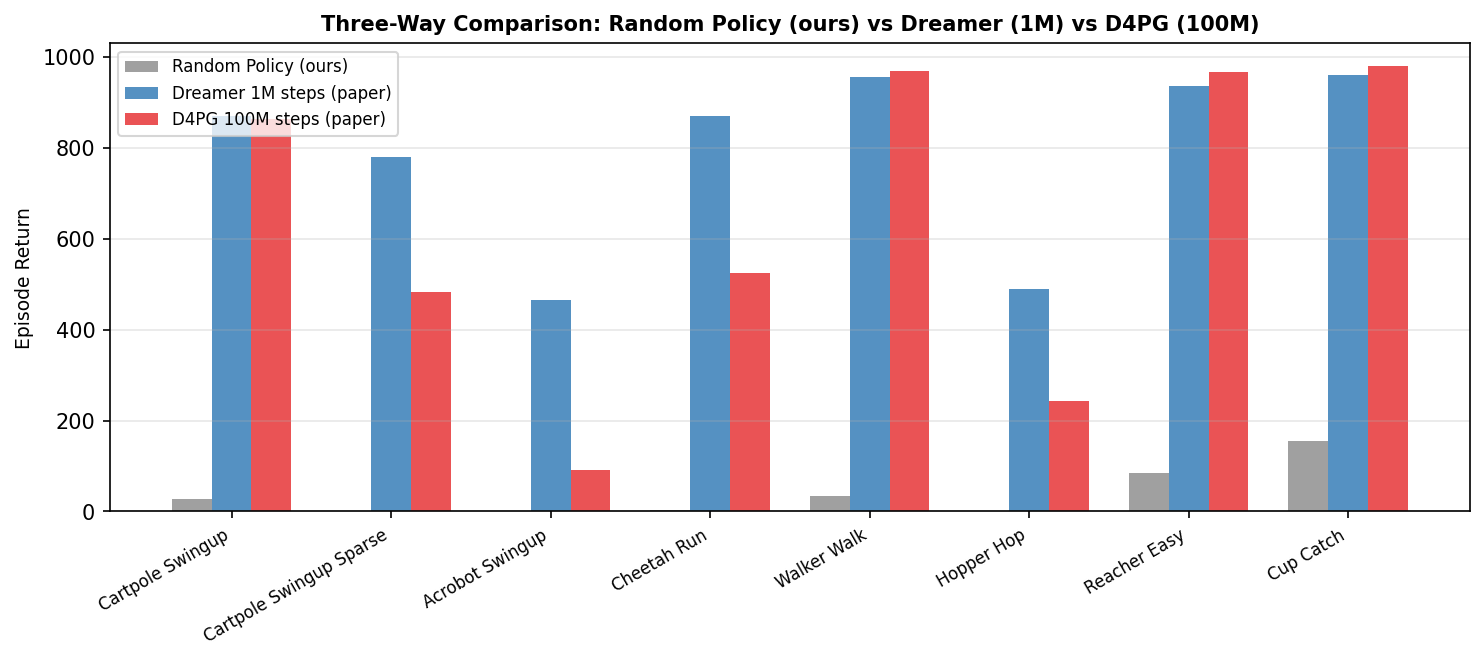
\includegraphics[width=\columnwidth]{fig1_three_way.png}
  \caption{Three-way comparison (our experiments): random policy (grey),
  Dreamer 1M steps (blue, paper), D4PG 100M steps (red, paper).
  Random baseline implements M2 \S2.1 (missing lower bound).}
  \label{fig:three_way}
\end{figure}

\begin{figure}[t]
  \centering
  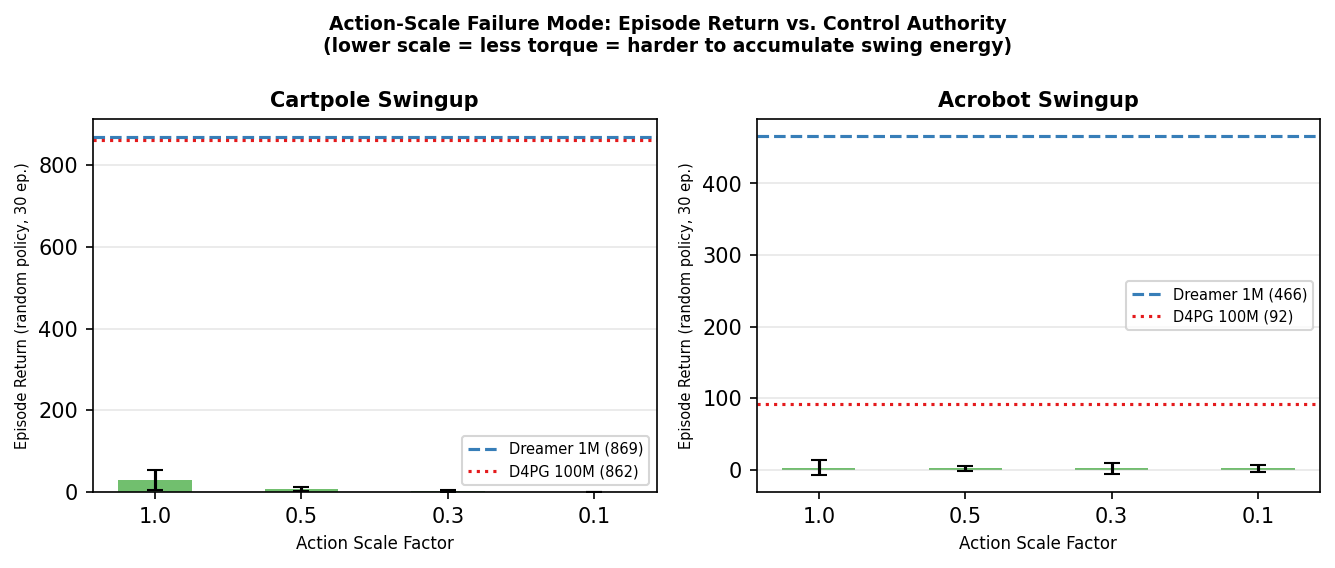
\includegraphics[width=\columnwidth]{fig2_action_scale.png}
  \caption{Action-scale failure mode (our experiment, 30 episodes each):
  return vs.\ control authority at scales 1.0, 0.5, 0.3, 0.1.
  Implements the energy-accumulation failure identified in M2
  feedback.}
  \label{fig:action_scale}
\end{figure}

\begin{figure}[t]
  \centering
  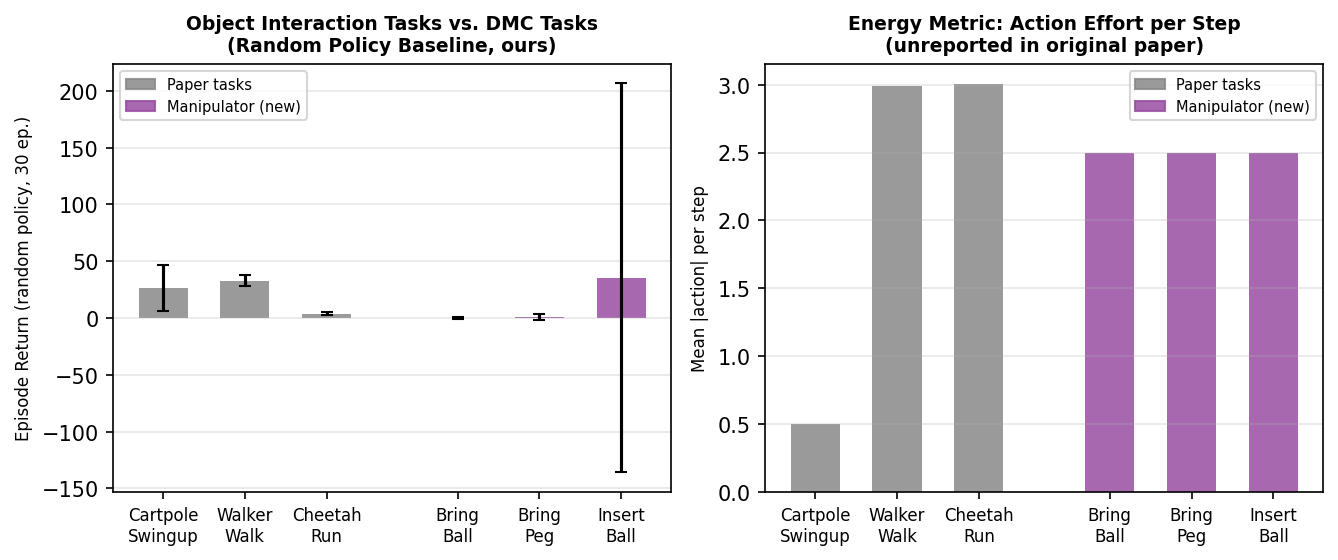
\includegraphics[width=\columnwidth]{fig3_manipulator_energy.png}
  \caption{Left: random-policy return on paper tasks (grey) vs.\
  manipulator tasks (purple), our experiment.  Right: energy metric
  (mean~$|a|$ per step)---unreported in paper.  Implements
  M2 \S3.2 (object interaction) and the energy metric from feedback.}
  \label{fig:manip}
\end{figure}

\begin{thebibliography}{9}
  \small
  \bibitem{dreamer} D.\ Hafner et al., ``Dream to Control: Learning
  Behaviors by Latent Imagination,'' \textit{ICLR 2020}.
  \bibitem{bestpractices} H.\ Kress-Gazit et al., ``Robot Learning as
  an Empirical Science: Best Practices for Policy Evaluation,''
  \textit{arXiv:2409.09491}, 2024.
  \bibitem{dmcontrol} Y.\ Tassa et al., ``dm\_control: Software
  package for physics-based simulation and RL,'' \textit{arXiv:2006.12983}, 2020.
\end{thebibliography}

\end{document}
